\documentclass[11pt,]{article}
\usepackage{lmodern}
\usepackage{amssymb,amsmath}
\usepackage{ifxetex,ifluatex}
\usepackage{fixltx2e} % provides \textsubscript
\ifnum 0\ifxetex 1\fi\ifluatex 1\fi=0 % if pdftex
  \usepackage[T1]{fontenc}
  \usepackage[utf8]{inputenc}
\else % if luatex or xelatex
  \ifxetex
    \usepackage{mathspec}
  \else
    \usepackage{fontspec}
  \fi
  \defaultfontfeatures{Ligatures=TeX,Scale=MatchLowercase}
\fi
% use upquote if available, for straight quotes in verbatim environments
\IfFileExists{upquote.sty}{\usepackage{upquote}}{}
% use microtype if available
\IfFileExists{microtype.sty}{%
\usepackage{microtype}
\UseMicrotypeSet[protrusion]{basicmath} % disable protrusion for tt fonts
}{}
\usepackage[margin=1in]{geometry}
\usepackage{hyperref}
\hypersetup{unicode=true,
            pdftitle={Analyse et prédiction des permis de construction en résidentiel},
            pdfauthor={Justine Mao, Nikita Gusarov, Tom Viellescazes},
            pdfborder={0 0 0},
            breaklinks=true}
\urlstyle{same}  % don't use monospace font for urls
\usepackage{graphicx,grffile}
\makeatletter
\def\maxwidth{\ifdim\Gin@nat@width>\linewidth\linewidth\else\Gin@nat@width\fi}
\def\maxheight{\ifdim\Gin@nat@height>\textheight\textheight\else\Gin@nat@height\fi}
\makeatother
% Scale images if necessary, so that they will not overflow the page
% margins by default, and it is still possible to overwrite the defaults
% using explicit options in \includegraphics[width, height, ...]{}
\setkeys{Gin}{width=\maxwidth,height=\maxheight,keepaspectratio}
\IfFileExists{parskip.sty}{%
\usepackage{parskip}
}{% else
\setlength{\parindent}{0pt}
\setlength{\parskip}{6pt plus 2pt minus 1pt}
}
\setlength{\emergencystretch}{3em}  % prevent overfull lines
\providecommand{\tightlist}{%
  \setlength{\itemsep}{0pt}\setlength{\parskip}{0pt}}
\setcounter{secnumdepth}{0}
% Redefines (sub)paragraphs to behave more like sections
\ifx\paragraph\undefined\else
\let\oldparagraph\paragraph
\renewcommand{\paragraph}[1]{\oldparagraph{#1}\mbox{}}
\fi
\ifx\subparagraph\undefined\else
\let\oldsubparagraph\subparagraph
\renewcommand{\subparagraph}[1]{\oldsubparagraph{#1}\mbox{}}
\fi

%%% Use protect on footnotes to avoid problems with footnotes in titles
\let\rmarkdownfootnote\footnote%
\def\footnote{\protect\rmarkdownfootnote}

%%% Change title format to be more compact
\usepackage{titling}

% Create subtitle command for use in maketitle
\providecommand{\subtitle}[1]{
  \posttitle{
    \begin{center}\large#1\end{center}
    }
}

\setlength{\droptitle}{-2em}

  \title{Analyse et prédiction des permis de construction en résidentiel}
    \pretitle{\vspace{\droptitle}\centering\huge}
  \posttitle{\par}
  \subtitle{Projet tutoré}
  \author{Justine Mao, Nikita Gusarov, Tom Viellescazes}
    \preauthor{\centering\large\emph}
  \postauthor{\par}
      \predate{\centering\large\emph}
  \postdate{\par}
    \date{20 février 2019}

\usepackage{setspace}

% to make the first rows bold in tables
\usepackage{longtable}
\usepackage{tabu}
\usepackage{booktabs}

% Floats
\usepackage{morefloats}
\usepackage{float}
\usepackage{placeins}

% highlighting
\usepackage{soul}

% Short toc
\usepackage{shorttoc}
\setcounter{tocdepth}{1}

% referencing mutliple things with a single command - \cref
\usepackage{cleveref}

% longtables
\usepackage{longtable}

% Change section names style
\usepackage[dvipsnames]{xcolor}
% \usepackage{sectsty}

% \sectionfont{\color{Green}}  % sets colour of sections
% \subsectionfont{\color{Green}}  % sets colour of sub
% \subsubsectionfont{\color{Green}}  % sets colour of subsub

% this makes dots in table of contents
% \renewcommand{\cftsecleader}{\cftdotfill{\cftdotsep}}
% to change the title of contents
% \renewcommand{\contentsname}{Whatever}

% line numbers for review purposes
% this package might not be available in default latex installation 
% get it by 'sudo tlmgr install lineno'
%\usepackage{lineno}
%\linenumbers

% Array
\usepackage{array}

% Multiple columns
\usepackage{multicol}

% Image insertion and colors
\usepackage{graphicx}

% to be able to include latex comments
\newenvironment{dummy}{}{}

% maketitle definition
\makeatletter
\def\@maketitle{
    \pagenumbering{gobble}
    \raggedright
    \includegraphics[height = 40mm]{../images/logouga.png} \quad
    \includegraphics[height = 40mm]{../images/logoshnd.jpg}
    \begin{center}
        \vspace*{\fill}
            {\Huge \color{Green} \@title}\\
            \par
            \rule{5cm}{0.4pt}
            \par
            %\textbf{Rapport de stage}\\[10mm]
            {\Large \@author}\\[10mm]
        \vspace*{\fill}
    \end{center}
    {\large Tuteur universitaire: }\\
    \hspace{10mm} {\large Béatrice Roussillon}\\
    {\large Tuteur de l'entreprise: }\\
    \hspace{10mm} {\large Mathias Verdiere}\\
    \vspace{10mm}
    {\large Niveau d'études : }\\
    \hspace{10mm} {\large Master 2}\\
    {\large Parcours : }\\
    \hspace{10mm} {\large Chargé d'études économiques et statistique}\\
    \vspace{20mm}
    \begin{center}
        {\large Université Grenoble Alpes}\\
        {\large Faculté d'économie et gestion}\\
        \vspace{5mm}
        2019 - 2020\\
    \end{center}
    \clearpage
}
\makeatother

\begin{document}
\maketitle


\hypersetup{linkcolor = black}
\pagenumbering{roman}

\tableofcontents

% \newpage

% % list of figures have to be added manually to table of contents
% \listoffigures 

% \newpage
% \listoftables

% \doublespacing

\newpage

\pagenumbering{arabic}
\hypersetup{linkcolor = blue}

\hypertarget{introduction}{%
\section{Introduction}\label{introduction}}

Le marché du bâtiment a une place prépondérante dans l'économie
française. Un des premiers secteurs d'activité économique (Gallay,
2017), le secteur du bâtiment et des travaux publics (nommé BTP)
disposait d'un chiffre d'affaires s'élevant à 170 milliards d'euros en
2016. La filière du bâtiment devrait voir évoluer sa croissance à la
hausse dans les années à venir. Selon une étude de Xerfi, l'institut
d'études privé, cette croissance est due d'une part à la rénovation
énergétique et d'autre part aux nouveaux programmes immobiliers. Le
marché du bâtiment se décompose en trois branches si on se base sur les
codes NAF : le marché de la construction spécialisée, le marché de la
construction et de la promotion immobilière, le marché du génie civil et
des travaux publics. Nous allons ici se pencher sur l'étude de la
construction et de la promotion immobilière. Sa part dans le chiffre
d'affaires total était de 23.8\% en 2016. Cette branche se concentre sur
la construction de bâtiments résidentiels et non résidentiels. La
recherche académique dans le domaine du bâtiment est florissante. De
nombreux travaux se sont penchés sur le domaine du BTP notamment dans le
résidentiel pour comprendre l'évolution de la construction. Etudier
l'évolution des autorisations de chantier nécessite de prendre en compte
le contexte macroéconomique afin de limiter tout biais. La Fédération
française du bâtiment (2017) ont identifié empiriquement une corrélation
entre les variables macroéconomiques et le nombre de permis de
construire : plus le taux des obligations assimilables au Trésor à 10
ans (OAT) augmente, plus le nombre de permis de construire est bas,
toutes choses égales par ailleurs. Lindh et al.~(2002) ajoutent qu'il
est important d'étudier aussi l'évolution du PIB. En effet, lorsque la
croissance économique du pays augmente, la corrélation devient positive,
toutes choses égales par ailleurs. Tandis que l'impact des variables
macroéconomiques sur le nombre de permis de construire semble faire
l'objet d'un certain consensus, la question sur le lien entre l'âge de
la population et le nombre d'autorisations de chantier peut être
intéressante à étudier (Essafi et al, 2013). Etant donné l'état actuel
de la recherche, l'objectif de notre projet est de comparer nos
estimations des nombres de permis de construire dans le résidentiel avec
celles trouvées par les cabinets privés.

De quelle manière peut-on estimer le nombre de permis de construire dans
le résidentiel ?

Le marché du bâtiment, spécialement le secteur résidentiel-tertiaire,
fait parti des filières qui consomme le plus d'énergie à l'échelle
européenne. L'efficacité énergétique des bâtiments est une problématique
importante du point de vue de Schneider. Il est donc intéressant ici de
se pencher sur l'évolution de la construction afin de trouver des
solutions à la crise énergétique. Pour analyser la relation entre les
variables macroéconomiques et le nombre de permis de construire, le
rapport est structuré comme suit. La section II mettra l'accent sur la
revue de la littérature. Dans la section III, nous présenterons le plan
d'analyse. Les résultats économétriques seront analysés dans la section
IV. La conclusion est présentée dans la dernière section.

\hypertarget{presentation-de-lentreprise}{%
\section{Présentation de
l'entreprise}\label{presentation-de-lentreprise}}

Présentation de l'entreprise Schneider Electric est une multinationale
française de gestion et d'automatisation de l'énergie. Acteur majeur de
la gestion de l'énergie, il a réalisé 27,7 milliards d'euros de chiffre
d'affaires en 2018. Elle a été créée en 1838, se manifestant sur le
marché de l'acier avant de se réorienter vers le marché de l'électricité
qui est devenu son cœur de métier dans les années 80. Le groupe
diversifie ses activités par différents segments de marché:

\begin{itemize}
\tightlist
\item
  Segment commercial

  \begin{itemize}
  \tightlist
  \item
    Bâtiments résidentiels, industriels et commerciaux (40\%);
  \item
    Centres de recherche (14\%);
  \end{itemize}
\item
  Infrastructure et industrie

  \begin{itemize}
  \tightlist
  \item
    Industrie (29\%);
  \item
    Entreprises d'infrastructures et d'électricité (17\%).
  \end{itemize}
\end{itemize}

En tant que société multinationale, Schneider Electric est présente dans
plus de 100 pays à travers le monde avec plus de 142 milliers
d'employés. La part du chiffre d'affaires par zone géographique montre
une différenciation équilibrée des activités:

\begin{itemize}
\tightlist
\item
  Amérique du Nord (28\%);
\item
  Europe occidentale (27\%);
\item
  Asie-Pacifique (29\%);
\item
  Reste du monde (16\%).
\end{itemize}

Aujourd'hui, les solutions Schneider sont adoptées dans plus de 450 000
systèmes dans le monde. Acteur majeur sur le marché des systèmes
énergétiques, Schneider contribue au développement durable mondial en se
fixant des objectifs élevés afin de préserver notre planète.

\hypertarget{revue-de-la-literature-economiques}{%
\section{Revue de la litérature
économiques}\label{revue-de-la-literature-economiques}}

Nous avons commencé notre étude de la littérature par la recherche des
articles méthodologiques et théoriques en lien avec le sujet traité.

Les ressources informatiques offertes par notre établissement
(Université Grenoble Alpes) aussi bien que d'autres sources en libre
accès nous ont permis de rechercher les articles d'intérêt. Les moteurs
de recherche scientifique les plus utilisés ont été : - Science Direct -
Google Scholar - Elsevier - SAGE journals Ces outils informatiques nous
ont permis de sélectionner les articles les plus pertinents selon le
nombre des citations des articles.

\hypertarget{synthese}{%
\subsection{Synthèse}\label{synthese}}

Les caractéristiques générales de l'économie et de la société peuvent
influencer l'évolution des permis de construire dans le résidentiel.
Avant d'aller plus loin, il n'est sans doute pas inutile de rappeler en
quelques mots ce que l'on entend généralement par le mot permis de
construire. Un permis de construire est ``un document administratif qui
donne les moyens à l'administration de vérifier qu'un projet de
construction respecte bien les règles d'urbanisme en vigueur. Ce
document obligatoire pour les travaux de grande importance ne doit
porter que sur les biens immobiliers'' (Walscheid). Plusieurs facteurs
déterminent le macro-environnement des permis de construire tels que les
facteurs économiques (croissance économiques, chômage), les facteurs
démographiques (l'évolution de la pyramide des âges) ainsi que les
facteurs politiques et légaux. De nombreux travaux ont cherché à faire
un état des lieux sur le nombre des autorisations de chantier dans le
résidentiel. Ils vont nous permettre de nous aiguiller sur le choix des
variables, leur unité ainsi que la méthode économétrique à appliquer.

\newpage

\begin{longtable}{p{5cm} | p{5cm} | p{5cm}}
\\[-1.8ex]
\hline \\[-1.8ex]
\textbf{Variables explicatives possibles} &
    \textbf{Pourquoi ? Théories} & 
        \textbf{Effet attendu sur la variable dépendante} \\
\hline \\[-1.8ex]
Nombre de permis de construire des logements décalé d’un trimestre (Fédération française du bâtiment, 2017) &
    L’évolution des permis de construire décalée d’un trimestre ne devrait pas changer soudainement d’un trimestre à un autre. Si le nombre d’autorisations de chantier décalé d’un trimestre augmente, on s’attend à ce que le nombre de permis de construire augmente par la suite, toutes choses égales par ailleurs. & 
        Effet positive \\
\hline \\[-1.8ex]
Taux de l’OAT à 10 ans décalé de deux trimestres (Fédération française du bâtiment, 2017) & 
    Si le taux de l’OAT augmente, les taux des crédits immobiliers le seront également. Les individus vont moins recourir à des crédits ce qui par la suite conduit à une baisse de la construction des bâtiments. Le nombre de permis de construire va donc diminuer. &
        Effet négative \\
\hline \\[-1.8ex]
Taux de chômage décalé de deux trimestres (Fédération française du bâtiment, 2017) & 
    Si le taux de chômage augmente d’1%, les individus possèdent moins d’argent et n’ont pas forcément la possibilité d’acheter un nouvel appartement. Le nombre de permis de construire devrait donc diminuer, toutes choses égales par ailleurs. & 
        Effet négative \\
\hline \\[-1.8ex]
Délai d’écoulement de l’encours de logements en trimestre de ventes décalés d’un trimestre (Fédération française du bâtiment, 2017) & 
    Plus le délai du crédit accordé à un client pour l’achat d’un logement s’allonge, plus le nombre de permis de construire va diminuer. En effet, les individus vont d’abord finir de rembourser leur crédit avant d’acheter un nouvel appartement. Plus ils tardent à rembourser, moins il y aura de demandes sur le marché de l’immobilier. & 
        Effet négative \\
\hline \\[-1.8ex]
Mesure politique & 
    La loi de finances a diminué les recettes des bailleurs sociaux ce qui par la suite, a aussi entraîné une baisse de l’investissement dans la construction de bâtiments neufs. Cela signifie en d’autres termes une baisse des autorisations de chantier, toutes choses égales par ailleurs. & 
        Effet positive ou négative selon la politique mise en place. \\
\hline \\[-1.8ex]
Âge de la population (Lindh et al, 2008) &
    Cela peut s’expliquer par un modèle de demande de cycle de vie en forme de bosse au cours de l’âge. Le taux de mortalité en augmentation à cet âge là constitue une partie importante de l’explication. Compte tenu du vieillissement rapide de la population dans les pays industrialisés, on peut s’attendre à une baisse des autorisations de chantier. & 
        Un effet positive pour les individus âgés entre 20 et 59 ans (Institut national d’études démographiques, 2019). Un effet négative pour les individus âgés de plus de 75 ans. \\
\hline \\[-1.8ex]
Prix de l’immobilier (Essai et al, 2015) &
    Celui-ci peut influencer indirectement le nombre de permis de construire. En effet, si le prix de l’immobilier augmente, les individus seront moins enclins à acheter des appartements. On peut s’attendre par la suite à ce que le nombre de permis de construire diminue. &
        Effet négative \\
\hline \\[-1.8ex]
PIB (Lindh et al, 2002) & 
    Plus la croissance est forte, plus le pays est riche. Les salaires des individus augmentent et vont se mettre à plus consommer. La demande de nouveaux logements augmente ainsi que les permis de construire. & 
        Effet positive. \\
\hline \\[-1.8ex]
\caption{Tableau récapitulatif des variables explicatives possibles du modèle}
\end{longtable}

From
\url{https://www.sciencedirect.com/science/article/abs/pii/S0164070407000997}
(Policy implications =\textgreater{} find monetary chocs) : Galbraith
and Tkacz (2007)

Overall, the results indicate that housing starts and residential
investment respond negatively to contractionary monetary policy shocks.
However, the magnitude of the impact is sensitive to the selection of
the horizon for which the restrictions hold. Moreover, a comparison of
the results with those obtained from a conventional Choleski
decomposition, suggests that the impact of monetary policy on the
housing market is much less certain under the sign restrictions
approach.

From
\url{https://www.sciencedirect.com/science/article/abs/pii/S0094119012000575}
(housing driven buiseness cycle) :

building permits significantly lead economic activity in nearly all US
states over the past three decades, and produce substantially more
accurate out-of-sample forecasts of state-level job and income growth
than other traditional indicators including the leading indicator index,
housing prices and wealth. housing reflects expectations of future
economic activity as permits are closely related to movements in
consumer expectations, and both lead the business cycle by four
quarters.

From \url{https://ideas.repec.org/p/bca/bocawp/05-41.html} :

The long-run relationship between expenditure and its determinants is
shown to have shifted during the late 1970s, which implies that
important changes have occurred in how the housing market is driven. The
author finds that the response of housing investment to interest rates
has become more pronounced over time. He compares out-of-sample
forecasts from linear and non-linear cointegration models (which make
use of information on fundamentals such as wealth and demographics) with
forecasts from simple leading-indicator models (which exploit
information such as housing starts or household indebtedness). The
author finds that simple leading-indicator models can provide relatively
accurate near-term forecasts. The preferred structural model, which
allows for a shift in the cointegrating vector, provides a rich analysis
of the housing sector, with good forecast accuracy on the construction
side but not on the resale side, which is more difficult to predict.

\hypertarget{plan-danalyse}{%
\section{Plan d'analyse}\label{plan-danalyse}}

\hypertarget{creation-dune-base-de-donnees}{%
\subsection{Création d'une base de
données}\label{creation-dune-base-de-donnees}}

Notre étude porte sur des données annuelles afin d'obtenir des résultats
sur le long terme.

Pour tester notre modèle économique, nous allons utiliser plusieurs
variables. La variable d'intérêt est le nombre de logements autorisés à
la construction dans le résidentiel en nombre de logements. Les
variables explicatives sont le PIB (en millions d'euros que nous
transformerons par la suite en indice base 1994), le taux d'inflation
(en indice base 1994), la part de la population par âge (âge), les
politiques publiques instaurées ainsi que l'année (variable binaire qui
prendra 1 lorsque nous étudierons cette année sinon 0).

L'étude à réaliser est dynamique puisque les données varient d'une année
à une autre.

Pour la collecte de nos données, nous nous sommes appuyés de plusieurs
sources : Eurostat, Data.gouv ainsi que l'Insee. Eurostat est un
fournisseur de statistiques qui exploite des données à l'échelle
européenne. Il ne collecte pas les données mais les vérifie afin de
veiller à leur comparabilité. Les chiffres sur Eurostat nous ont permis
d'avoir des données sur le secteur de la construction. Data.gouv.fr est
une ``plateforme de diffusion de données publiques'' en France. Nous
pouvons retrouver sur cette plateforme les bases de données Sitadel2 qui
recensent les permis de construire. L'Insee produit, analyse et publie
les données statistiques en France. Il nous a permis de disposer des
informations sur les variables macro-économiques ainsi que les taux
d'intérêt.

\hypertarget{methodologie}{%
\section{Methodologie}\label{methodologie}}

\hypertarget{les-predictions-et-les-limitations}{%
\subsection{Les prédictions et les
limitations}\label{les-predictions-et-les-limitations}}

From
\url{https://ideas.repec.org/a/aea/jecper/v12y1998i2p175-92.html\#author-abstract}
:

Broadly defined, macroeconomic forecasting is alive and well.
Nonstructural forecasting, which is based largely on reduced-form
correlations, has always been well and continues to improve. Structural
forecasting, which aligns itself with economic theory and hence rises
and falls with theory, receded following the decline of Keynesian
theory. In recent years, however, powerful new dynamic stochastic
general equilibrium theory has been developed and structural
macroeconomic forecasting is poised for resurgence.

From Bank of Canada Working Paper 2007, 1,
\url{https://www.econstor.eu/handle/10419/53936} :

For stationary transformations of variables, there exists a maximum
horizon beyond which forecasts can provide no more information about the
variable than is present in the unconditional mean. Meteorological
forecasts, typically excepting only experimental or exploratory
situations, are not reported beyond this horizon; by contrast, little
generally accepted information about such maximum horizons is available
for economic variables. The authors estimate such content horizons for a
variety of economic variables, and compare these with the maximum
horizons that they observe reported in a large sample of empirical
economic forecasting studies. The authors find that many published
studies provide forecasts exceeding, often by substantial margins, their
estimates of the content horizon for the particular variable and
frequency. The authors suggest some simple reporting practices for
forecasts that could potentially bring greater transparency to the
process of making and interpreting economic forecasts.

\hypertarget{donnees}{%
\section{Données}\label{donnees}}

Notre étude porte à la fois sur les données annuelles et mensuelles, ce
qui vise d'enrichir et raffiner notre analyse par une exploration des
interactions du court et long terme. Néanmoins, suivant le contexte de
notre étude, ainsi bien que les demandes du commanditaire, nous allons
nous focaliser surtout sur les données annuelles, car Schnieder
Electrics est intéressé par des résultats ayant une valeur stratégique
au long terme.

Notre base des données regroupe des indices macroéconomiques provenant
de plusieurs sources français et internationaux. Parmi lesquels :

\begin{itemize}
\tightlist
\item
  Eurostat ;
\item
  Base des données gouvernementale
  \href{mailto:Sit@del2}{\nolinkurl{Sit@del2}} ;
\item
  Insee.
\end{itemize}

Les variables récupérées de ces base des données sont :

\begin{itemize}
\tightlist
\item
  Nombre des logements autorisés à la construction,
\item
  La surface autorisée à la construction,
\item
  Produit intérieur brut,
\item
  Taux d'inflation,
\item
  Données sur les parts de la population par âge,
\item
  Données sur les politiques publiques mises en place.
\end{itemize}

\FloatBarrier

\begin{table}[!htbp] \centering 
\begin{tabular}{@{\extracolsep{5pt}}lcccc} 
\\[-1.8ex]\hline 
\hline \\[-1.8ex] 
Statistic & \multicolumn{1}{c}{Mean} & \multicolumn{1}{c}{St. Dev.} & \multicolumn{1}{c}{Min} & \multicolumn{1}{c}{Max} \\ 
\hline \\[-1.8ex] 
Année & 2,006.000 & 7.360 & 1,994 & 2,018 \\ 
PIB & 1,956.328 & 219.289 & 1,545.800 & 2,285.900 \\ 
Taux d'intérêt & 3.903 & 1.867 & 0.468 & 7.535 \\ 
Depences des ménages & 1,018.228 & 122.541 & 801.300 & 1,186.200 \\ 
Investissements des ménages & 111.336 & 12.820 & 87.300 & 134.800 \\ 
Nombre des logements autorisé & 381,173.600 & 70,800.620 & 275,711 & 526,592 \\ 
Mettres quarrés autorisés & 36,530,295.000 & 7,069,575.000 & 26,739,099 & 52,443,730 \\ 
Population < 20 ans & 25.007 & 0.686 & 24.003 & 26.370 \\ 
Population 20-59 ans & 52.887 & 1.389 & 49.991 & 54.176 \\ 
Population > 60 ans & 22.105 & 1.964 & 19.882 & 26.006 \\ 
\hline \\[-1.8ex] 
\end{tabular} 
  \caption{Statistiques déscriptives pour les données annuelles} 
  \label{} 
\end{table}

\FloatBarrier

\hypertarget{transformation-des-donnees}{%
\subsection{Transformation des
données}\label{transformation-des-donnees}}

Afin de pouvoir traiter les données recueillis nous devons les rapporter
à une échelle commune afin d'éviter les biais éventuelles liées à la
présence d'héterockedacité. Nous ajustons les données en les ramenant à
la base de 1994. C'est-à-dire, nous construisons des indice pour toutes
les séries temporelles.

Les statistiques descriptives pour les données transformées sont
présentés dans le tableau suivant :

\FloatBarrier

\begin{table}[!htbp] \centering 
\begin{tabular}{@{\extracolsep{5pt}}lcccc} 
\\[-1.8ex]\hline 
\hline \\[-1.8ex] 
Statistic & \multicolumn{1}{c}{Mean} & \multicolumn{1}{c}{St. Dev.} & \multicolumn{1}{c}{Min} & \multicolumn{1}{c}{Max} \\ 
\hline \\[-1.8ex] 
Année & 12.000 & 7.360 & 0 & 24 \\ 
PIB & 1.266 & 0.142 & 1 & 1 \\ 
Taux d'intérêt & 0.541 & 0.259 & 0.065 & 1.045 \\ 
Depences des ménages & 1.271 & 0.153 & 1 & 1 \\ 
Investissements des ménages & 1.275 & 0.147 & 1 & 2 \\ 
Nombre des logements autorisé & 1.208 & 0.224 & 1 & 2 \\ 
Population < 20 ans & 0.948 & 0.026 & 1 & 1 \\ 
Population 20-59 ans & 0.984 & 0.026 & 1 & 1 \\ 
Population > 60 ans & 1.112 & 0.099 & 1 & 1 \\ 
Mettres quarrés autorisés & 1.227 & 0.237 & 1 & 2 \\ 
\hline \\[-1.8ex] 
\end{tabular} 
  \caption{Statistiques déscriptives pour les données annuelles transorfmées} 
  \label{} 
\end{table}

\FloatBarrier

\hypertarget{presentation-graphique}{%
\subsection{Présentation graphique}\label{presentation-graphique}}

Afin de pouvoir mieux comprendre le comportement des différents séries
temporelles nous pouvons visualiser nos données. Cette représentation
devra nous donner une intuition sur les problèmes éventuelles (telles
que la non-stationnarité).

\FloatBarrier

\begin{figure}[!htbp]

{\centering \includegraphics{rapport_files/figure-latex/unnamed-chunk-15-1} 

}

\caption{Les données originales}\label{fig:unnamed-chunk-15}
\end{figure}

\FloatBarrier

Puisque nous faisons face à des séries chronologiques annuelles nous
évitons les obstacles imposées par la structure saisonnière des données.
Néanmoins, un nombre d'observation faible, ainsi que la présence des
tendances temporelles nous complexifient notre analyse.

\hypertarget{analyse-de-la-correlation}{%
\subsection{Analyse de la correlation}\label{analyse-de-la-correlation}}

\hypertarget{analyse-simple}{%
\subsubsection{Analyse simple}\label{analyse-simple}}

Nous allons commencer par une presentation simple etudiant la
corremation entre les variables étudiées sans prendre en compte les
decalages temporaires.

\hypertarget{analyse-des-correlations-croisees}{%
\subsubsection{Analyse des corrélations
croisées}\label{analyse-des-correlations-croisees}}

D'ici nous introduisons dans notre analyse la notion des liens causales
dans le temps. Afin de pouvoir capter les rélations sous-jacents dans
nos données nous allons étudier les correlations croisées entre les
variables identifiées.

Toutefois, avant d'utiliser cette téchnique nous devons nous assurer sur
la stationnaritée des séries étudiées. Afin de reussir dans cette tache,
nous effectuons deux tests :

\begin{itemize}
\tightlist
\item
  test de Dickey-Fuller augmenté (ADF), qui permet de tester l'hypothèse
  de la non-stationnarité d'une série temporelle ;
\item
  test de Kwiatkowski-Phillips-Schmidt-Shin (KPSS) pour vérifier la
  stationnarité sur trend (KPSS-T) ou niveau (KPSS-L).
\end{itemize}

Ces deux tests nous permettent de vérifier l'hypothèse de la
staionnarité des séries étudiées et, si besoin, la corriger en
appliquant une transformation sur la série en question.

\FloatBarrier

\begin{table}[ht]
\centering
\begin{tabular}{rrrr}
  \hline
 & ADF & KPSS.T & KPSS.L \\ 
  \hline
PIB & 0.59 & 0.01 & 0.01 \\ 
  Taux d'inflation & 0.24 & 0.10 & 0.01 \\ 
  Depences des ménages & 0.79 & 0.01 & 0.01 \\ 
  Investissements des ménages & 0.63 & 0.02 & 0.05 \\ 
  Nombre des logements autorisé & 0.36 & 0.08 & 0.08 \\ 
  Population $<$ 20 ans & 0.67 & 0.01 & 0.01 \\ 
  Population 20-59 ans & 0.53 & 0.01 & 0.01 \\ 
  Population $>$ 60 ans & 0.48 & 0.01 & 0.01 \\ 
   \hline
\end{tabular}
\caption{Tests de la stationnaritée, p-valeurs} 
\end{table}

\FloatBarrier

Les résultats obtenus pour le test de Dickey-Fuller nous permetent
rejeter l'hypothèse de la stationnarité des séries temporelles en
question. De même, selon les résultats d'autre test (KPSS) nous devons
rejeter l'hypothèse de stationnarité soit sur trend, soit sur niveau
pour l'ensemble des données.

Nous observons dans nos données (graphique X) que les séries temporelles
n'oscille pas autour du zero, ce qui, tenant compte des résultats des
tests, nous amêne à l'idée que nos séries sont stationnaires en
differences. Cela nous amêne à des séries résultantes suivantes :

\FloatBarrier

\begin{figure}[!htbp]

{\centering \includegraphics{rapport_files/figure-latex/unnamed-chunk-19-1} 

}

\caption{Les données differenciées}\label{fig:unnamed-chunk-19}
\end{figure}

\FloatBarrier

Vérifions si ces séries sont stationnaires. Effectuons les tests, qu'on
a déjà utilisé :

\FloatBarrier

\begin{table}[ht]
\centering
\begin{tabular}{rrrr}
  \hline
 & ADF & KPSS.T & KPSS.L \\ 
  \hline
PIB & 0.30 & 0.10 & 0.10 \\ 
  Taux d'inflation & 0.06 & 0.10 & 0.10 \\ 
  Depences des ménages & 0.05 & 0.10 & 0.10 \\ 
  Investissements des ménages & 0.42 & 0.10 & 0.10 \\ 
  Nombre des logements autorisé & 0.01 & 0.10 & 0.10 \\ 
  Population $<$ 20 ans & 0.56 & 0.10 & 0.04 \\ 
  Population 20-59 ans & 0.68 & 0.10 & 0.02 \\ 
  Population $>$ 60 ans & 0.54 & 0.10 & 0.02 \\ 
   \hline
\end{tabular}
\caption{Tests de la stationnaritée en differences, p-valeurs} 
\end{table}

\FloatBarrier

Dans ce cas, nous obtenons des résultats satisfaisants au moins pour un
certain nombre des séries étudiées. Ce qui est le plus importent, c'est
que la série principale décrivant l'evolution du nombre des logements
autorisé est stationnaire en prémiers differences.

\FloatBarrier

\begin{figure}[!htbp]

{\centering \includegraphics{rapport_files/figure-latex/unnamed-chunk-22-1} 

}

\caption{Corremogrammes croisées}\label{fig:unnamed-chunk-22}
\end{figure}

\FloatBarrier

Nous observons, que pour l'ensemble des données on n'arrive pas capter
les liens causales, car la correlation observé sur notre échantillon est
plus forte au temps 0 (en abcense du décalage temporaire entre les deux
séries dans chaque cas).

Il existe en même temps une faible correlation négative entre le taux
d'interêt décalé et le nombre des logements autorisé. C'est-à-dire, une
augmentation du taux d'intérêt risque d'entrainer une baisse dans le
nobmre des autorisations de construction (il faut ne pas oublier qu'ici
on parle des valeurs differenciées et pas des nombres réels). D'utre
coté, l'augmentation des autorisations à construire entraine une hausse
de PIB (dans ce cas la correlation observée est trop faible, mais
significative tout de même).

\FloatBarrier

\begin{figure}[!htbp]

{\centering \includegraphics{rapport_files/figure-latex/unnamed-chunk-23-1} 

}

\caption{Corremogrammes croisées}\label{fig:unnamed-chunk-23}
\end{figure}

\FloatBarrier

Nous observons une forte correlation entre le nombre des logements
autorisé à la construction dans le secteur privé et la part de la
population mineur de 20 ans, ce qui s'explique par l'idée des cycles de
vie, qui apparait dans un des articles étudiées.

\hypertarget{autocorrelation}{%
\subsection{Autocorrelation}\label{autocorrelation}}

\FloatBarrier

\begin{figure}[!htbp]

{\centering 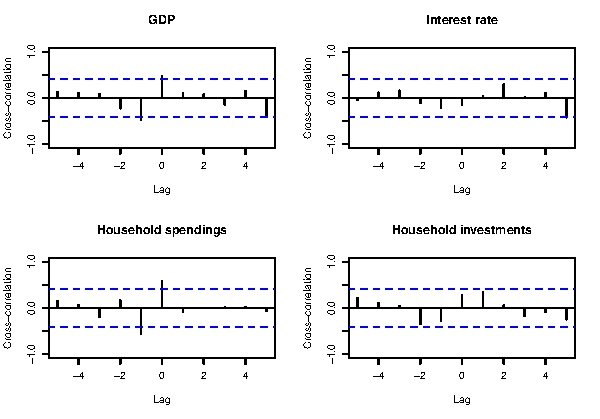
\includegraphics{rapport_files/figure-latex/unnamed-chunk-24-1} 

}

\caption{Corremogrammes croisées}\label{fig:unnamed-chunk-24}
\end{figure}

\FloatBarrier

\FloatBarrier

\begin{figure}[!htbp]

{\centering 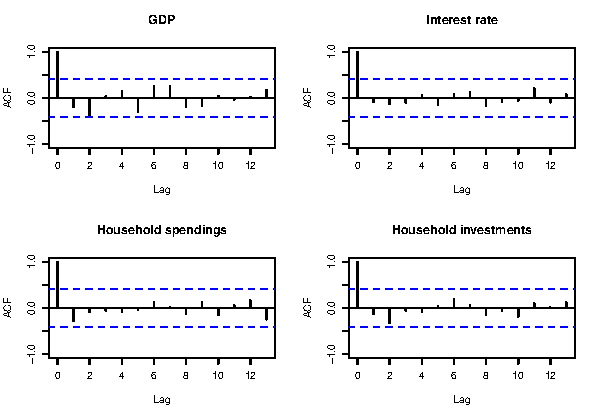
\includegraphics{rapport_files/figure-latex/unnamed-chunk-25-1} 

}

\caption{Corremogrammes croisées}\label{fig:unnamed-chunk-25}
\end{figure}

\FloatBarrier

\hypertarget{autocorrelation-partielle}{%
\subsection{Autocorrelation partielle}\label{autocorrelation-partielle}}

\FloatBarrier

\begin{figure}[!htbp]

{\centering 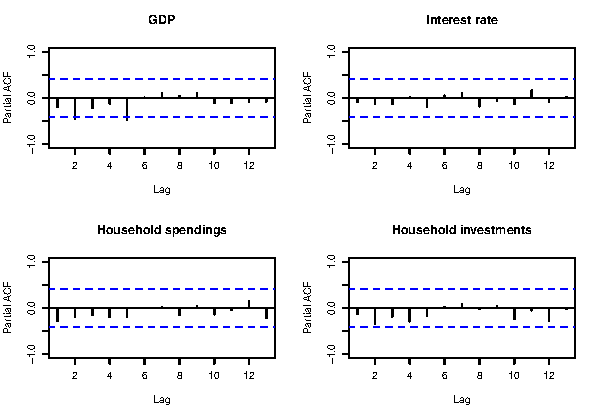
\includegraphics{rapport_files/figure-latex/unnamed-chunk-26-1} 

}

\caption{Corremogrammes croisées}\label{fig:unnamed-chunk-26}
\end{figure}

\FloatBarrier

\FloatBarrier

\begin{figure}[!htbp]

{\centering \includegraphics{rapport_files/figure-latex/unnamed-chunk-27-1} 

}

\caption{Corremogrammes croisées}\label{fig:unnamed-chunk-27}
\end{figure}

\FloatBarrier

\hypertarget{modelisation}{%
\section{Modèlisation}\label{modelisation}}

Dans cette partie nous allons discuter des différents approches à la
prédiction de nombre des logement autorisé à la construction. A l'aide
de plusieurs modèles intermédiaires nous allons démontrer la meilleure
façon à traiter la problématique.

\ldots{}

\hypertarget{annexes}{%
\section{Annexes}\label{annexes}}

\hypertarget{a-modeles-econometriques-simples}{%
\subsection{A Modèles économétriques
simples}\label{a-modeles-econometriques-simples}}

Dans cette partie de travail nous allons explorer préalablement les
liens éventuels entre nos variables par construction d'une régression
simple.

\FloatBarrier

\begin{table}[!htbp]
\begin{center}
\begin{tabular}{l c c c c c }
\hline
 & Model 1 & Model 2 & Model 3 & Model 4 & Model 5 \\
\hline
PIB            & $0.99^{***}$ & $-0.64$     & $1.67^{*}$ & $-3.70$      & $-5.58$    \\
               & $(0.26)$     & $(2.31)$    & $(0.66)$   & $(3.00)$     & $(3.71)$   \\
Taux d'interet &              &             & $0.37$     & $-0.67$      & $-0.52$    \\
               &              &             & $(0.35)$   & $(0.38)$     & $(0.42)$   \\
FBCFmen        &              & $1.18^{**}$ &            & $1.73^{***}$ & $2.51^{*}$ \\
               &              & $(0.31)$    &            & $(0.44)$     & $(1.00)$   \\
Temps          &              &             &            &              & $0.06$     \\
               &              &             &            &              & $(0.07)$   \\
\hline
R$^2$          & 0.39         & 0.64        & 0.42       & 0.69         & 0.70       \\
Adj. R$^2$     & 0.36         & 0.59        & 0.36       & 0.62         & 0.62       \\
Num. obs.      & 25           & 25          & 24         & 24           & 24         \\
RMSE           & 0.18         & 0.14        & 0.18       & 0.14         & 0.14       \\
\hline
\multicolumn{6}{l}{\scriptsize{$^{***}p<0.001$, $^{**}p<0.01$, $^*p<0.05$}}
\end{tabular}
\caption{Comparaison des modèles differents}
\label{table:coefficients}
\end{center}
\end{table}

\FloatBarrier

\hypertarget{b-modeles-temporelles-simples}{%
\subsection{B Modéles temporelles
simples}\label{b-modeles-temporelles-simples}}

\FloatBarrier

\begin{figure}[!htbp]

{\centering \includegraphics{rapport_files/figure-latex/unnamed-chunk-34-1} 

}

\caption{Graphiques déscriptives 1}\label{fig:unnamed-chunk-34}
\end{figure}

\FloatBarrier

\FloatBarrier

\begin{figure}[!htbp]

{\centering \includegraphics{rapport_files/figure-latex/unnamed-chunk-35-1} 

}

\caption{Graphiques déscriptives 2}\label{fig:unnamed-chunk-35}
\end{figure}

\FloatBarrier

\FloatBarrier

\begin{table}[!htbp]
\begin{center}
\begin{tabular}{l c c c c c }
\hline
 & Model 1 & Model 2 & Model 3 & Model 4 & Model 5 \\
\hline
ar1            & $0.11$   &          & $-0.95$  & $0.49$   &          \\
               & $(0.20)$ &          & $(0.23)$ & $(0.23)$ &          \\
intercept      & $0.01$   & $0.01$   & $0.01$   & $0.01$   & $0.01$   \\
               & $(0.04)$ & $(0.04)$ & $(0.03)$ & $(0.01)$ & $(0.03)$ \\
ma1            &          & $0.15$   & $0.93$   & $-0.69$  &          \\
               &          & $(0.21)$ & $(0.27)$ & $(0.24)$ &          \\
ma2            &          &          &          & $-0.31$  &          \\
               &          &          &          & $(0.20)$ &          \\
\hline
AIC            & -11.46   & -11.60   & -9.30    & -12.34   & -13.19   \\
Log Likelihood & 8.73     & 8.80     & 8.65     & 11.17    & 8.59     \\
\hline
\multicolumn{6}{l}{\scriptsize{$^{***}p<0.001$, $^{**}p<0.01$, $^*p<0.05$}}
\end{tabular}
\caption{Comparaison des modèles ARMA}
\label{table:coefficients}
\end{center}
\end{table}

\FloatBarrier

\hypertarget{modeles-temporelles-de-type-var}{%
\subsection{Modèles temporelles de type
VAR}\label{modeles-temporelles-de-type-var}}

\FloatBarrier

\begin{table}[!htbp]
\begin{center}
\begin{tabular}{l c c c c c c c c }
\hline
 & rPIB & rTdI & rDCFmen & rFBCFmen & rTNL & rmoins20 & rmid2059 & rplus60 \\
\hline
rPIB.l1     & $-1.05$  & $-3.38$     & $-0.42$    & $-2.23$    & $-13.12$    & $0.02$   & $0.06$      & $-0.19$       \\
            & $(0.61)$ & $(2.14)$    & $(0.45)$   & $(1.64)$   & $(6.15)$    & $(0.05)$ & $(0.07)$    & $(0.15)$      \\
rTdI.l1     & $-0.01$  & $-0.21$     & $0.02$     & $-0.13$    & $0.56$      & $-0.01$  & $-0.00$     & $0.02$        \\
            & $(0.07)$ & $(0.23)$    & $(0.05)$   & $(0.18)$   & $(0.67)$    & $(0.01)$ & $(0.01)$    & $(0.02)$      \\
rDCFmen.l1  & $0.42$   & $5.07^{**}$ & $0.33$     & $0.91$     & $-1.11$     & $-0.03$  & $0.01$      & $0.00$        \\
            & $(0.39)$ & $(1.36)$    & $(0.29)$   & $(1.05)$   & $(3.93)$    & $(0.03)$ & $(0.04)$    & $(0.10)$      \\
rFBCFmen.l1 & $0.28$   & $1.21$      & $0.06$     & $0.50$     & $1.73$      & $-0.00$  & $-0.02$     & $0.05$        \\
            & $(0.17)$ & $(0.58)$    & $(0.12)$   & $(0.45)$   & $(1.68)$    & $(0.01)$ & $(0.02)$    & $(0.04)$      \\
rTNL.l1     & $0.03$   & $-0.09$     & $0.00$     & $0.16^{*}$ & $0.33$      & $-0.00$  & $-0.00$     & $0.00$        \\
            & $(0.02)$ & $(0.09)$    & $(0.02)$   & $(0.07)$   & $(0.25)$    & $(0.00)$ & $(0.00)$    & $(0.01)$      \\
rmoins20.l1 & $4.06$   & $-3.34$     & $4.59$     & $6.56$     & $78.30^{*}$ & $0.16$   & $0.23$      & $-0.83$       \\
            & $(3.04)$ & $(10.70)$   & $(2.27)$   & $(8.21)$   & $(30.83)$   & $(0.25)$ & $(0.33)$    & $(0.75)$      \\
rmid2059.l1 & $-0.65$  & $-5.57$     & $1.94$     & $6.42$     & $14.29$     & $-0.01$  & $0.90^{**}$ & $-2.41^{***}$ \\
            & $(2.14)$ & $(7.54)$    & $(1.60)$   & $(5.79)$   & $(21.71)$   & $(0.17)$ & $(0.23)$    & $(0.53)$      \\
const       & $0.06$   & $-0.18$     & $0.05^{*}$ & $0.07$     & $0.86^{*}$  & $-0.00$  & $-0.00$     & $0.01$        \\
            & $(0.03)$ & $(0.11)$    & $(0.02)$   & $(0.08)$   & $(0.31)$    & $(0.00)$ & $(0.00)$    & $(0.01)$      \\
trend       & $-0.00$  & $0.00$      & $-0.00$    & $-0.00$    & $-0.02$     & $0.00$   & $-0.00$     & $0.00$        \\
            & $(0.00)$ & $(0.00)$    & $(0.00)$   & $(0.00)$   & $(0.01)$    & $(0.00)$ & $(0.00)$    & $(0.00)$      \\
\hline
R$^2$       & 0.54     & 0.67        & 0.53       & 0.71       & 0.53        & 0.59     & 0.88        & 0.89          \\
Adj. R$^2$  & 0.26     & 0.47        & 0.24       & 0.53       & 0.25        & 0.34     & 0.80        & 0.82          \\
Num. obs.   & 22       & 22          & 22         & 22         & 22          & 22       & 22          & 22            \\
RMSE        & 0.01     & 0.05        & 0.01       & 0.04       & 0.15        & 0.00     & 0.00        & 0.00          \\
\hline
\multicolumn{9}{l}{\scriptsize{$^{***}p<0.001$, $^{**}p<0.01$, $^*p<0.05$}}
\end{tabular}
\caption{Résultat de VAR(1)}
\label{table:coefficients}
\end{center}
\end{table}

\FloatBarrier

\FloatBarrier

\begin{table}[!htbp]
\begin{center}
\begin{tabular}{l c c c c c c c c }
\hline
 & rPIB & rTdI & rDCFmen & rFBCFmen & rTNL & rmoins20 & rmid2059 & rplus60 \\
\hline
rPIB.l1     & $-1.26$  & $-4.31$     & $-0.28$  & $-3.17$   & $-11.78$     & $0.05$      & $-0.04$  & $0.03$   \\
            & $(1.18)$ & $(2.72)$    & $(0.53)$ & $(2.92)$  & $(6.62)$     & $(0.05)$    & $(0.10)$ & $(0.30)$ \\
rTdI.l1     & $0.03$   & $-0.08$     & $-0.04$  & $0.04$    & $-0.40$      & $-0.01$     & $0.01$   & $-0.01$  \\
            & $(0.14)$ & $(0.31)$    & $(0.06)$ & $(0.34)$  & $(0.76)$     & $(0.01)$    & $(0.01)$ & $(0.03)$ \\
rDCFmen.l1  & $0.87$   & $5.48^{**}$ & $0.41$   & $2.21$    & $-2.10$      & $0.01$      & $-0.02$  & $0.04$   \\
            & $(0.57)$ & $(1.31)$    & $(0.25)$ & $(1.41)$  & $(3.20)$     & $(0.03)$    & $(0.05)$ & $(0.15)$ \\
rFBCFmen.l1 & $0.25$   & $1.26$      & $-0.05$  & $0.35$    & $1.45$       & $-0.01$     & $0.01$   & $-0.01$  \\
            & $(0.36)$ & $(0.84)$    & $(0.16)$ & $(0.90)$  & $(2.03)$     & $(0.02)$    & $(0.03)$ & $(0.09)$ \\
rTNL.l1     & $0.00$   & $-0.21$     & $-0.02$  & $0.17$    & $0.29$       & $-0.01^{*}$ & $0.01$   & $-0.01$  \\
            & $(0.04)$ & $(0.10)$    & $(0.02)$ & $(0.10)$  & $(0.23)$     & $(0.00)$    & $(0.00)$ & $(0.01)$ \\
rmoins20.l1 & $7.22$   & $-3.86$     & $3.02$   & $22.63$   & $118.76^{*}$ & $0.11$      & $0.88$   & $-2.51$  \\
            & $(8.12)$ & $(18.70)$   & $(3.62)$ & $(20.11)$ & $(45.53)$    & $(0.36)$    & $(0.71)$ & $(2.08)$ \\
rmid2059.l1 & $4.45$   & $11.25$     & $2.57$   & $15.98$   & $6.75$       & $0.33$      & $0.57$   & $-1.98$  \\
            & $(4.32)$ & $(9.95)$    & $(1.92)$ & $(10.70)$ & $(24.22)$    & $(0.19)$    & $(0.38)$ & $(1.10)$ \\
rPIB.l2     & $-0.74$  & $-5.47$     & $-0.72$  & $0.84$    & $0.11$       & $-0.13^{*}$ & $0.21$   & $-0.39$  \\
            & $(1.02)$ & $(2.35)$    & $(0.45)$ & $(2.53)$  & $(5.72)$     & $(0.04)$    & $(0.09)$ & $(0.26)$ \\
rTdI.l2     & $0.01$   & $0.34$      & $-0.06$  & $-0.08$   & $-0.32$      & $0.01$      & $0.00$   & $-0.01$  \\
            & $(0.13)$ & $(0.30)$    & $(0.06)$ & $(0.32)$  & $(0.72)$     & $(0.01)$    & $(0.01)$ & $(0.03)$ \\
rDCFmen.l2  & $-0.36$  & $0.84$      & $0.20$   & $-1.08$   & $11.25^{*}$  & $-0.06$     & $-0.01$  & $0.10$   \\
            & $(0.70)$ & $(1.61)$    & $(0.31)$ & $(1.73)$  & $(3.92)$     & $(0.03)$    & $(0.06)$ & $(0.18)$ \\
rFBCFmen.l2 & $0.15$   & $0.98$      & $0.19$   & $-0.14$   & $-1.56$      & $0.03^{*}$  & $-0.05$  & $0.10$   \\
            & $(0.27)$ & $(0.62)$    & $(0.12)$ & $(0.67)$  & $(1.52)$     & $(0.01)$    & $(0.02)$ & $(0.07)$ \\
rTNL.l2     & $0.04$   & $0.19$      & $0.00$   & $0.11$    & $-0.14$      & $0.00$      & $-0.00$  & $0.00$   \\
            & $(0.04)$ & $(0.10)$    & $(0.02)$ & $(0.10)$  & $(0.23)$     & $(0.00)$    & $(0.00)$ & $(0.01)$ \\
rmoins20.l2 & $1.55$   & $12.32$     & $5.49$   & $-3.43$   & $21.64$      & $-0.09$     & $0.17$   & $-0.34$  \\
            & $(5.19)$ & $(11.95)$   & $(2.31)$ & $(12.85)$ & $(29.10)$    & $(0.23)$    & $(0.46)$ & $(1.33)$ \\
rmid2059.l2 & $-5.52$  & $-27.03$    & $-0.48$  & $-9.68$   & $25.36$      & $-0.22$     & $0.25$   & $-0.37$  \\
            & $(5.61)$ & $(12.92)$   & $(2.50)$ & $(13.89)$ & $(31.45)$    & $(0.25)$    & $(0.49)$ & $(1.43)$ \\
const       & $0.11$   & $0.08$      & $0.08$   & $0.15$    & $0.81$       & $-0.00$     & $0.00$   & $-0.01$  \\
            & $(0.10)$ & $(0.22)$    & $(0.04)$ & $(0.24)$  & $(0.54)$     & $(0.00)$    & $(0.01)$ & $(0.02)$ \\
trend       & $-0.00$  & $-0.01$     & $-0.00$  & $-0.00$   & $-0.02$      & $0.00$      & $-0.00$  & $0.00$   \\
            & $(0.00)$ & $(0.01)$    & $(0.00)$ & $(0.01)$  & $(0.02)$     & $(0.00)$    & $(0.00)$ & $(0.00)$ \\
\hline
R$^2$       & 0.76     & 0.91        & 0.91     & 0.87      & 0.93         & 0.94        & 0.96     & 0.94     \\
Adj. R$^2$  & 0.05     & 0.65        & 0.65     & 0.49      & 0.70         & 0.74        & 0.83     & 0.75     \\
Num. obs.   & 21       & 21          & 21       & 21        & 21           & 21          & 21       & 21       \\
RMSE        & 0.02     & 0.04        & 0.01     & 0.04      & 0.10         & 0.00        & 0.00     & 0.00     \\
\hline
\multicolumn{9}{l}{\scriptsize{$^{***}p<0.001$, $^{**}p<0.01$, $^*p<0.05$}}
\end{tabular}
\caption{Résultat de VAR(2)}
\label{table:coefficients}
\end{center}
\end{table}

\FloatBarrier

\hypertarget{references}{%
\section*{References}\label{references}}
\addcontentsline{toc}{section}{References}

\hypertarget{refs}{}
\leavevmode\hypertarget{ref-galbraith2007forecasting}{}%
Galbraith, John W., and Greg Tkacz. 2007. ``How Far Can Forecasting
Models Forecast? Forecast Content Horizons for Some Important
Macroeconomic Variables.'' Bank of Canada Working Paper 2007,1. Ottawa:
Bank of Canada. \url{http://hdl.handle.net/10419/53936}.


\end{document}
